\documentclass[16pt]{article}

\usepackage{lipsum} %dont know
\usepackage{geometry}
\geometry{top=2.5cm, left=2.6cm, right=2.1cm}
\usepackage{graphicx}
\usepackage{float}
\graphicspath{{images/}}
\usepackage{mathtools}
\usepackage{listings}
\lstset{language=Verilog, breaklines=true}
\usepackage{underscore}
\usepackage[utf8]{inputenc}



\begin{document}

\begin{titlepage}
  \begin{center}
  
\vspace*{0.5cm} 
  \Large{ISTANBUL TECHNICAL UNIVERSITY
COMPUTER ENGINEERING DEPARTMENT}

\vspace{2cm}
  \huge{\textbf{BLG222E}}\\
  \huge{\textbf{COMPUTER ORGANIZATION PROJECT 2 REPORT}}

\vspace{3cm}
  \Large{\textbf{Group Members:}}\\
  150200011 Çağla Mıdıklı\\
  150210049 Feyza Sarı\\
  820210305 Berna Karatay 
  
\vfill
  \Large{\textbf{24 MAY 2023}}  
  
  \end{center}

  \end{titlepage}

%contents 
\tableofcontents
\thispagestyle{empty}  
\clearpage
\setcounter{page}{1}

\section{Introduction}
In this project we designed hardwired control unit.


\section{Project or Materials and Methods}
\subsection{Timer Module}
The timer\_4\_bit module is a simple 4-bit timer that increments its output out on each positive clock edge. The value of out is controlled by the funsel input. When funsel is 0, out is set to 0, and when funsel is 1, out is incremented by 1.


\subsection{Hardwired Control Unit}
The hardwired control unit takes inputs from the ALU system and generates control signals and outputs for the computer. In this module inputs are reset, clock and IROut. ALU system inputs except RF\_TSel are outputs to hardwired control unit: !!aluflag
\begin{itemize}
    \item RF\_OutASel, RF\_OutBSel selects the source for Register File(RF) output A and B.
    \item RF\_FunSel selects the function to perform on the RF output.
    \item RF\_RSel selects the register to read from the RF.
    \item ALU\_FunSel, ALUFlag selects the ALU function and determines if ALU flags should be updated.
    \item ARF\_OutCSel, ARF\_OutDSel selects the source for the Arithmetic Register File(ARF) output C and D.
    \item ARF\_FunSel selects the function to perform on the ARF.
    \item ARF\_RegSel selects the register to write to in the ARF.
    \item IR\_LH, IR\_Enable, IR\_Funsel are control signals related to loading instructions from IR.
    \item Mem\_CS, Mem\_WR are control signals related to memory read/write operations.
    \item MuxASel, MuxBSel, MuxCSel are control signals for multiplexer selection.
\end{itemize}

In addition, there are output wires; addresing\_mode represents the addressing mode of the instruction,
regsel represents the register selection field of the instruction,
op\_address represents the operation address field of the instruction,
operation\_code represents the operation code field of the instruction.
Destination\_register, source\_register1, source\_register2 represents the register fields of the instruction.
Timer\_funsel and timer\_out are control signals and output of the 4-bit timer.


\subsubsection{OPCODE}

First of all, we loaded the destination register by applying the logic operations specified in this part to the source registers selected with the code.

ALU Logical Operation Part(opcode 0,1,2,3,4,5,6): According to the 16-bit data input operation is chosen as the logic operation to be carried out in alu. According to the 16-bit data input, we pick the rf registers used as source registers. We use the operation inside the alu. Afterwards, we load it into the destination register (RF-ARF is an option).

Register Operation Part(opcode 7,8): Alu chooses to do the logic operation on itself. According to the 16-bit data input, we discover the rf registers used as source registers. We make no internal changes to the alu. Afterwards, we load it into the final register (RF-ARF is an option). and we change the register's funsel to either raise or decrease the register we loaded by 1.

Loading Operation Part(opcode 9,10,11,12,13): Without doing any logical processes, we load the value from our input or registers into the target register in this section. We choose our source register based on the input's format and the value between the fifth and eighth bits.

SP Operation Part(opcode 14,15):The final step in this process firstly involves loading our SP register into our destination register and then raising its value by 1 for opcode 14. And we add one to our sp register's value before loading it into our destination register for opcode 15.


\subsection{Cpu}
In this portion, we combined the hardware unit and the alu system we produced in this assignment to make a straightforward computer that is capable of carrying out specific tasks.
\section{Results}
By entering various values into a testbench that we built, we were able to determine whether our code functions properly. When the necessary memory entries are present, our CPU completes the operations we require correctly.
\section{Discussion}
Reset input is provided at simulation's beginning, clearing RF, ARF, and IR. The first instruction, BRA 0x20 0420, is then loaded from memory at the beginning. Because it is loaded in partial, less significant part loads first and then at the following clock more significant half part loads. and then the source registers and destination registers we choose are selected according to the inputs we receive from the memory.
\section{Conclusion}
The register structure, its kinds, the operation of the ALU system, and the hardware control unit of a computer are all covered in this assignment. The CPU's structure was learned by us. While developing the Alu System, we had the chance to observe logical expressions as well as other extreme conditions (overflow, barrow, carry).


\begin{figure}[H]
    \centering
    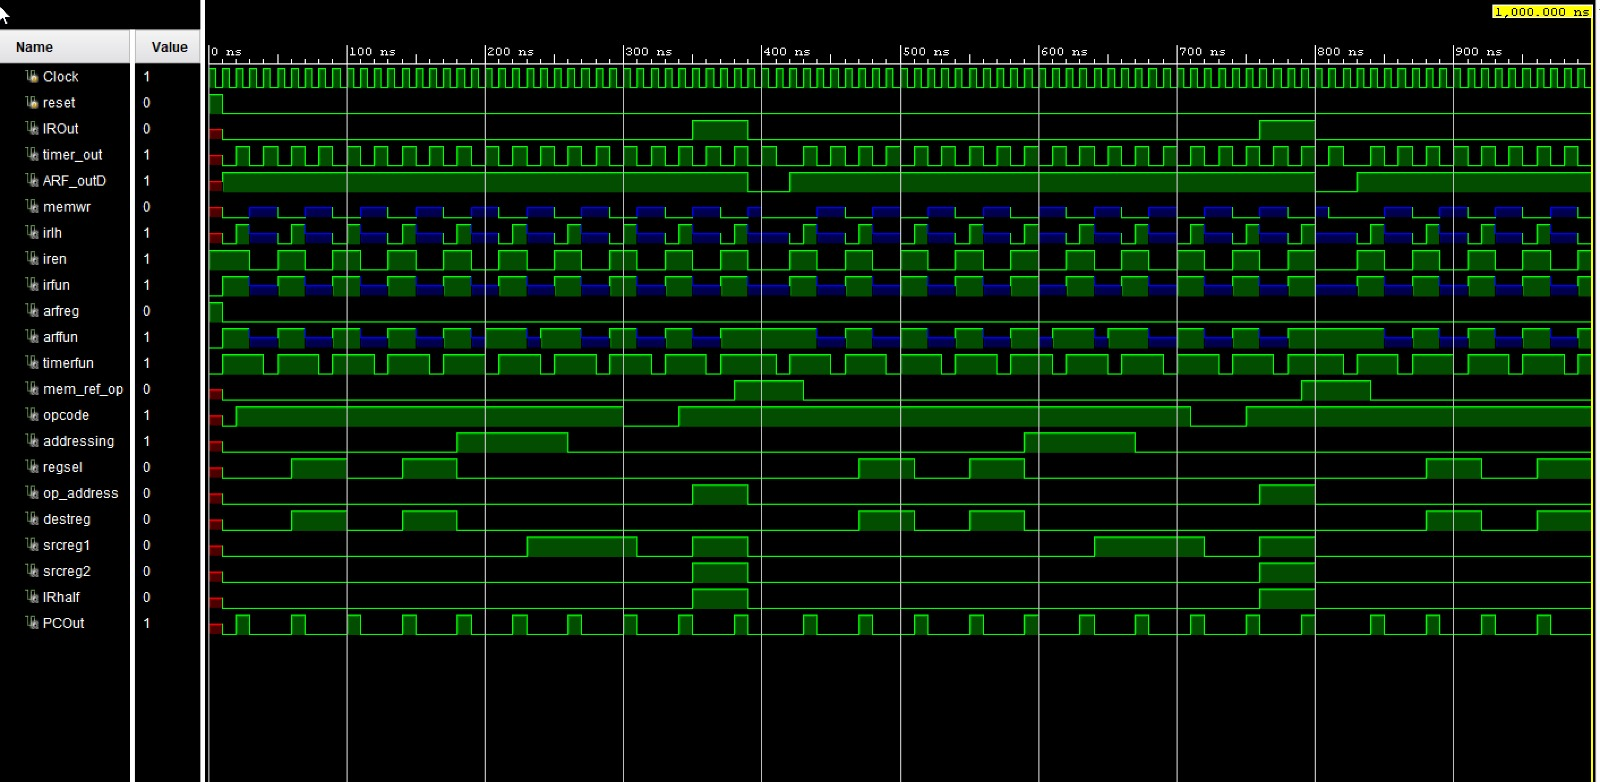
\includegraphics[width=6in]{hcu.jpg}
    \caption{Figure for part-2a}
    
\end{figure}






\end{document}